\documentclass[border=10pt]{standalone}

\usepackage{tikz}
\usepackage{tikzsymbols}
\usetikzlibrary{calc,patterns,shapes.geometric}

\def\centerarc[#1](#2)(#3:#4:#5){\draw[#1] ($(#2)+({#5*cos(#3)},{#5*sin(#3)})$) arc (#3:#4:#5);}

\begin{document}
	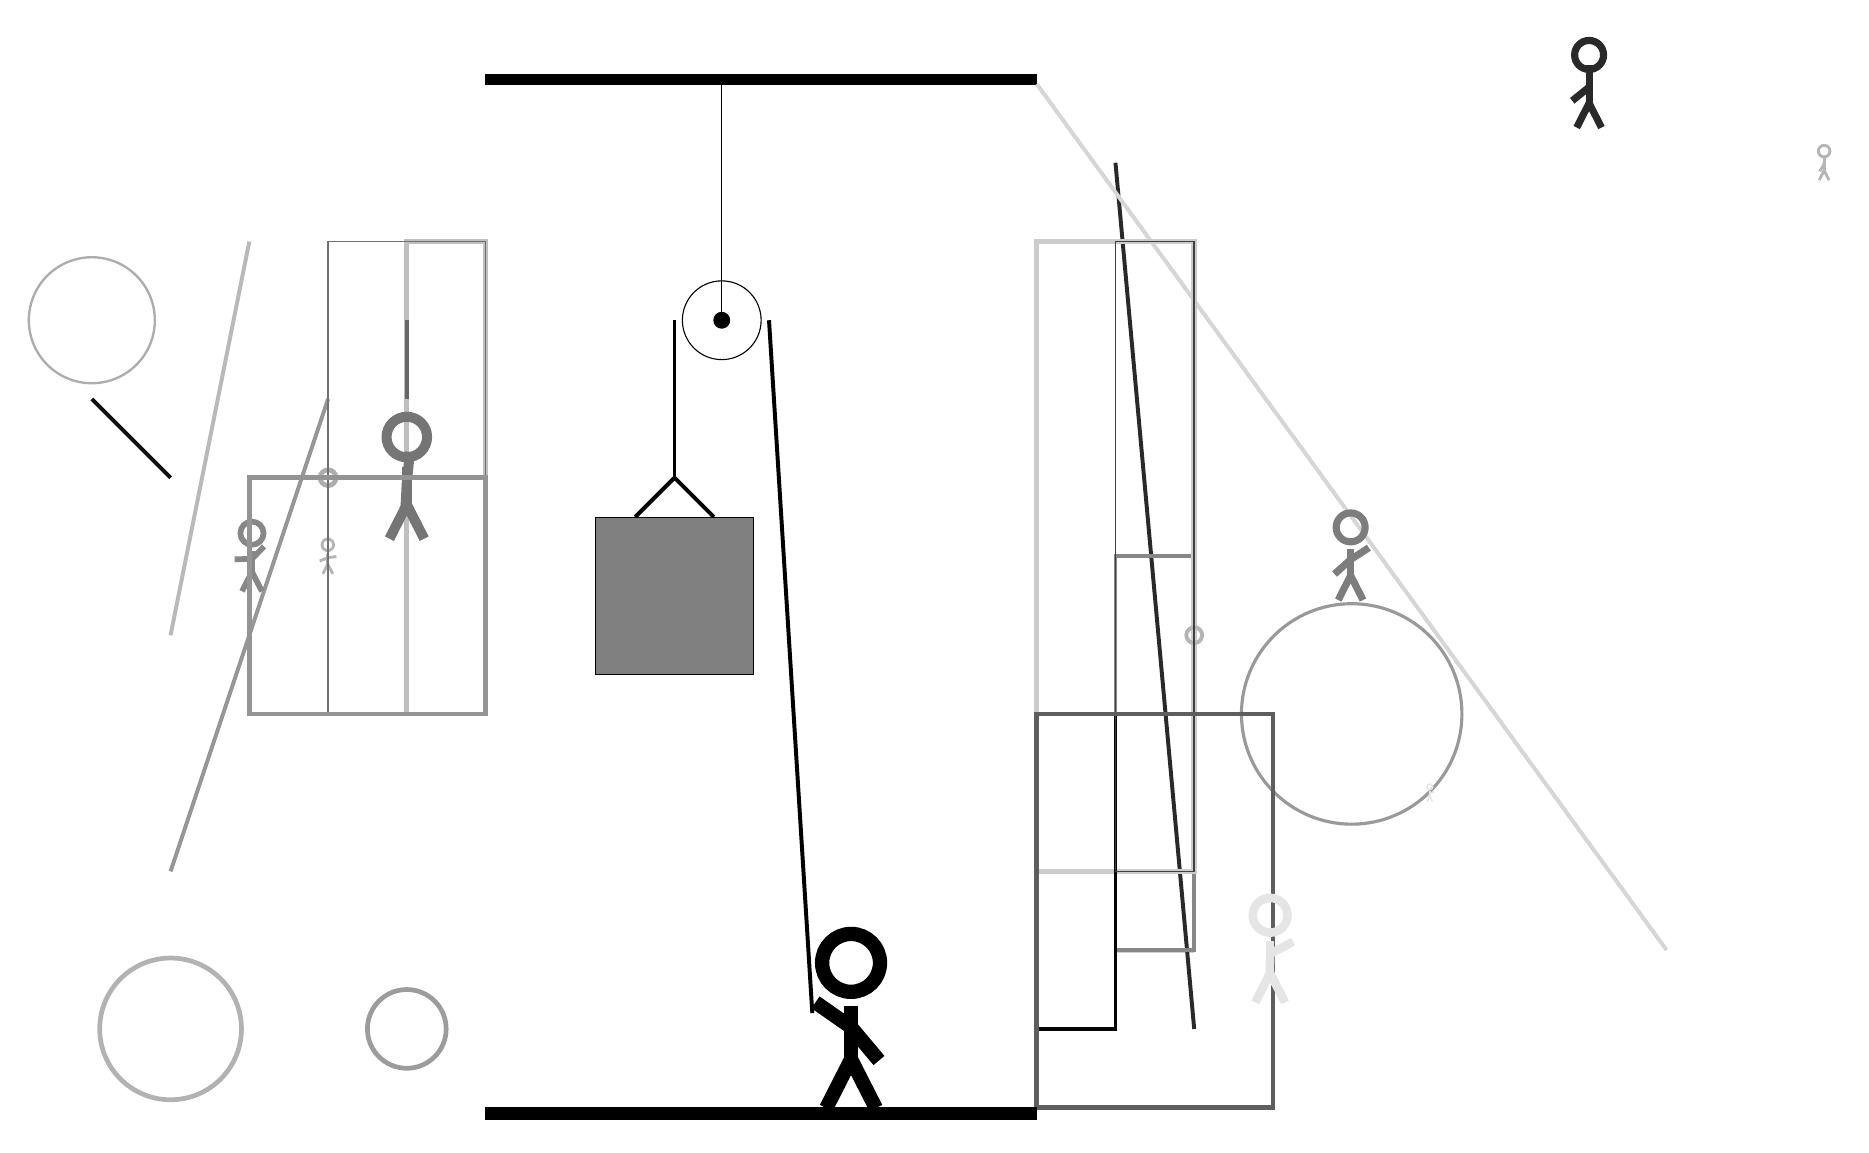
\begin{tikzpicture}
		%%%%% START %%%%%
		
		\draw[fill=black] (-2, 10) rectangle (5, 10.125);
		
		\draw (1, 7) circle (0.5);
		\draw[fill=black] (1, 7) circle (0.1);
		\draw (1, 10) -- (1, 7);
		
		\draw[line width=0.5mm] (-0.1, 4.5) -- (0.4, 5.0) -- (0.9, 4.5);
		\draw[fill=black!50] (-0.6, 4.5) rectangle (1.4, 2.5);
		
		\draw[line width=0.5mm] (0.4, 7) -- (0.4, 5.0);
		\centerarc[line width=0.5mm](1, 7)(0:180:0.6);
		\draw[line width=0.5mm](1.6, 7) -- (2.15, -1.8);
		
		\node at (2.6, -1.9) {\Strichmaxerl[10][-35][-50]};
		
		\draw [line width=0.4mm, color=black!40](9, 2) circle (1.4);
		
		\draw[line width=0.6mm, color=black!25] (-3, 8) rectangle (-2, 2);
		\draw[line width=0.6mm, color=black!18] (7, -1) rectangle (6, -1);
		\draw[line width=0.5mm, color=black!94](-7, 6) -- (-6, 5);
		
		\draw[line width=0.5mm, color=black!84](7, -2) -- (6, 9);
		\draw[line width=0.5mm, color=black!28](-5, 8) -- (-6, 3);
		\node[line width=0.7mm, color=black!29] at (-4, 4) {\Strichmaxerl[2][22][8]};
		\node[line width=0.6mm, color=black!29] at (15, 9) {\Strichmaxerl[2][59][84]};
		\node[line width=0.7mm, color=black!54] at (-3, 5) {\Strichmaxerl[7][87][84]};
		\draw[line width=0.5mm, color=black!47] (6, -1) rectangle (7, 4);
		\draw[line width=0.5mm, color=black!16](5, 10) -- (13, -1);
		
		\draw [line width=0.6mm, color=black!32](-4, 5) circle (0.1);
		\draw[line width=0.7mm, color=black!20] (5, 8) rectangle (7, 0);
		\draw[line width=0.5mm, color=black!99] (6, 2) rectangle (5, -2);
		\node[line width=0.2mm, color=black!10] at (10, 1) {\Strichmaxerl[1][68][20]};
		\draw [line width=0.5mm, color=black!29](7, 3) circle (0.1);
		
		\node[line width=0.2mm, color=black!84] at (12, 10) {\Strichmaxerl[5][39][90]};
		
		\draw [line width=0.3mm, color=black!32](-7, 7) circle (0.8);
		\draw[line width=0.2mm, color=black!75] (7, 8) rectangle (6, 0);
		\draw[line width=0.5mm, color=black!41](-4, 6) -- (-6, 0);
		\draw [line width=0.6mm, color=black!30](-6, -2) circle (0.9);
		\draw[line width=0.5mm, color=black!60](-3, 6) -- (-3, 7);
		
		\node[line width=0.7mm, color=black!51] at (9, 4) {\Strichmaxerl[5][42][33]};
		\draw[line width=0.2mm, color=black!56] (-2, 8) rectangle (-4, 2);
		\draw [line width=0.6mm, color=black!39](-3, -2) circle (0.5);
		
		\node[line width=0.3mm, color=black!47] at (-5, 4) {\Strichmaxerl[4][1][46]};
		\draw[line width=0.6mm, color=black!42] (-2, 2) rectangle (-5, 5);
		\draw[line width=0.6mm, color=black!63] (5, 2) rectangle (8, -3);
		\node[line width=0.6mm, color=black!10] at (8, -1) {\Strichmaxerl[6][89][28]};
		
		\draw[fill=black] (-2, -3) rectangle (5, -3.15);
		
		%%%%% END %%%%%
	\end{tikzpicture}
\end{document}